\begin{thm}{162}{\hosi 5}{京大プレ理系 2017第2回}
 曲線$y=\log x$ $(1\le x \le e)$ を$x$軸のまわりに1回転させてできる曲面を、$y$軸のまわりに1回転させてできる立体の体積を求めよ。
\end{thm}

体積を求める立体を$K$とし、その体積を$V$とする。曲線$y=\log x$ $(1\le x\le e)$を$x$軸で回転させたときの曲面は、
\begin{align*}
 \left\{
 \begin{aligned}
  y^2+z^2&=(\log x)^2 \\
  1\le x&\le e
 \end{aligned}
 \right.
\end{align*}
として表せる。この曲面は$xz$平面対称であるから$K$もそうであり、$K$のうち$y\ge 0$の部分の体積は$\dfrac{1}{2}V$である。

$K$は$-1\le y\le 1$の範囲に存在するので、$y=k$ $(0\le k\le 1)$で$K$を切断したときの断面を考える。上の曲面を$y=k$で切断した部分は ($xz$平面に射影すると)
\begin{align*}
 \left\{
 \begin{aligned}
  z^2&=(\log x)^2-k^2 \\
  e^k&\le x\le e
 \end{aligned}
 \right.
\end{align*}
という曲線になるので、これを$C_k$と呼ぶ。$C_k$上の点$\mathrm{P}$は、$\mathrm{P}(t,\pm\sqrt{(\log t)^2-k^2})$ と書くことができ (ただし$e^k\le t\le e$)、符号がいずれであっても原点との距離の2乗$D(t)$は
\[ D(t)=t^2+(\log t)^2-k^2 \]
となる。$D(t)$は明らかに$t$につれて増加するから、
\[ e^{2k}\le D(t)\le e^2+1-k^2 \]
であることがわかる。これは、$C_k$上で最も原点に近い点が$(e^{k},0)$であり、最も遠い点が$(e,\sqrt{1-k^2})$であることからくる。よって、$C_k$を原点中心に回転させると円環領域$e^k\le r\le \sqrt{e^2+1-k^2}$ になることが分かり、これが$K$の平面$y=k$での断面である。
\begin{figure}[H]
 \centering
 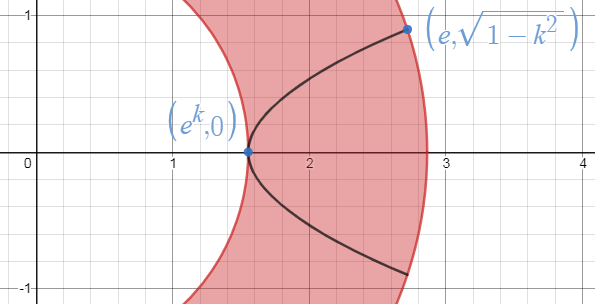
\includegraphics[width=0.8\linewidth]{../problems/Q_162/A_162.png}
\end{figure}
この断面積を$S(k)$とおくと、
\[ S(k)=\pi(e^2+1-k^2-e^{2k}) \]
となる。よって、
\begin{align*}
 \frac{1}{2}V&=\int_0^1\! S(y) \,dy \\
 &=\pi\Bigl[(e^1+1)y-\frac{1}{3}y^3-\frac{1}{2}e^{2y}\Bigr]_0^1 = \left(\frac{1}{2}e^2+\frac{7}{6}\right)\pi
\end{align*}
以上より、$V=\left(e^2+\dfrac{7}{3}\right)\pi$